\section{Current Implementations}
The current de facto standard for representing words in vector space is Word2vec. In this vector space each vector corresponds to a single word, these word vectors are contained in multidimensional space with their length and direction altered based on the words use in a given corpus. The creation of these vectors is a multi step process:
\begin{enumerate}
    \item Data Preparation - Define corpus, clean, normalise and tokenise words
    \item Hyper parameters - Learning rate, epochs, window size, embedding size
    \item Generate Training Data - Build vocabulary, one-hot encoding for words, build dictionaries that map id to word and vice versa
    \item Model Training - Pass encoded words through forward pass, calculate error rate, adjust weights using back propagation and compute loss
    \item Inference - Get word vector and find similar words
    \item Further improvements - Speeding up training time with Skip-gram Negative Sampling (SGNS) and Hierarchical Softmax
\end{enumerate}

\noindent
Word2vec can be trained in two ways Continuous Bag-Of-Words (CBOW) or continuous Skip-gram (SG). CBOW will attempt to guess the output; a single word from surrounding words and generally is faster to train. While SG will attempt to guess context words from a single word and tends to work better when a only a smaller corpus is available. This choice must be made at the begining of training and generally two models are created one for each method. \cite{Mikolov}

Word2vec has many strong use cases with a focus in information retrieval and knowledge discovery. One such example is where Word2vec was used to identify new chemical compounds based on specific properties. In this paper the training corpus was approximately 3.3 million abstracts from 1000 different journals. By looking at relations between different compounds using analogies learned during the training process. In this case Word2vec was integral in the training process, chemical formulae were included in normalised form and trained using skip-gram. The end result was the ability to enter a normalised formulae with the SG model returning a list of context words some of which being a property of the supplied compound such as thin, magnetic etc. \cite{Tshitoyan}

\section{Vector Combinations}
One of the strengths of Word2Vec is the ability to subtract two vectors and add the result to a third, allowing for another form of relationship between word vectors to appear. This concept is one of the best examples to show how Word2Vec can give the illusion that semantic understanding is built into the Word2Vec model. This concept was introduced in the original Word2vec paper by employees at Google in 2013 and includes some promising results.

\begin{figure}[h]
    \centering
    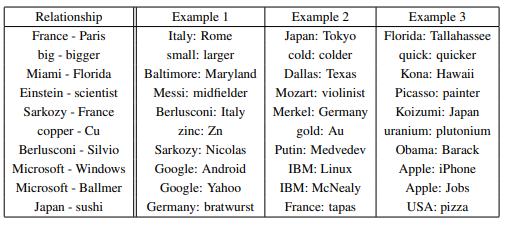
\includegraphics[]{images/learned_relationships}
    \caption{Word pair relationships}
    \label{fig:table_relations}
\end{figure}

\noindent
In figure ~\ref{fig:table_relations} the subtraction vectors appear in the left column and the addition vector is listed before the colon in each subsequent column. The resulting vector is then given, for example in the first row Paris is subtracted from France and Italy is added giving the result of Rome. In the original creation of Word2Vec this process was correct approximately 60\% of the time. \cite{Mikolova} It may be easy to say in figure 2 that the model has some sort of understanding of language as it provides logical results in figure ~\ref{fig:table_relations} however it is important to note that this understanding is extracted embedded \textit{meaning} within the corpus. Therefore this extraction of meaning may be biased based on the supplied corpus, and example of which was used to show the possibility that Amazons AI recruiting tool formed a bias against women. This bias appears to have formed from the data used and not from the model \cite{Caliskan}, in this paper Word2vec was used in combination with Glove. Glove, created in Stanford can be used to identify structure within the generated vector space and in this case was used to identify the bias embedded within the corpus. \cite{Pennington}

\section{Cosine Similarity}
 The representation of words as vectors can give the appearance of meaning in text using methods such as Word2Vec. This meaning can appear due to the way Word2Vec represents words vectors in high dimensional space. When the Word2Vec model is queried with two input vectors the vectors are found in the model and by calculating the cosine similarity between these two vectors a value between zero and one is obtained. Naturally the vector representation of words such as car and wall will have a value close to zero while wall and house will produce a value closer to one. This ability to obtain a value between zero and one for how similar two words allows for the extraction of basic meaning from text. 
 
 The cosine similarity allows for the abstraction of the length of the word vectors and instead will focus on the angle between said vectors. This idea overcomes the general approach of counting the most common words to tell if a document is similar or in the case when investigating words counting the common letters. This ability to ignore magnitude and focus on angles in multidimensional space allows for more meaningful relations to be found.
 
 \begin{figure}[h]
    \centering
    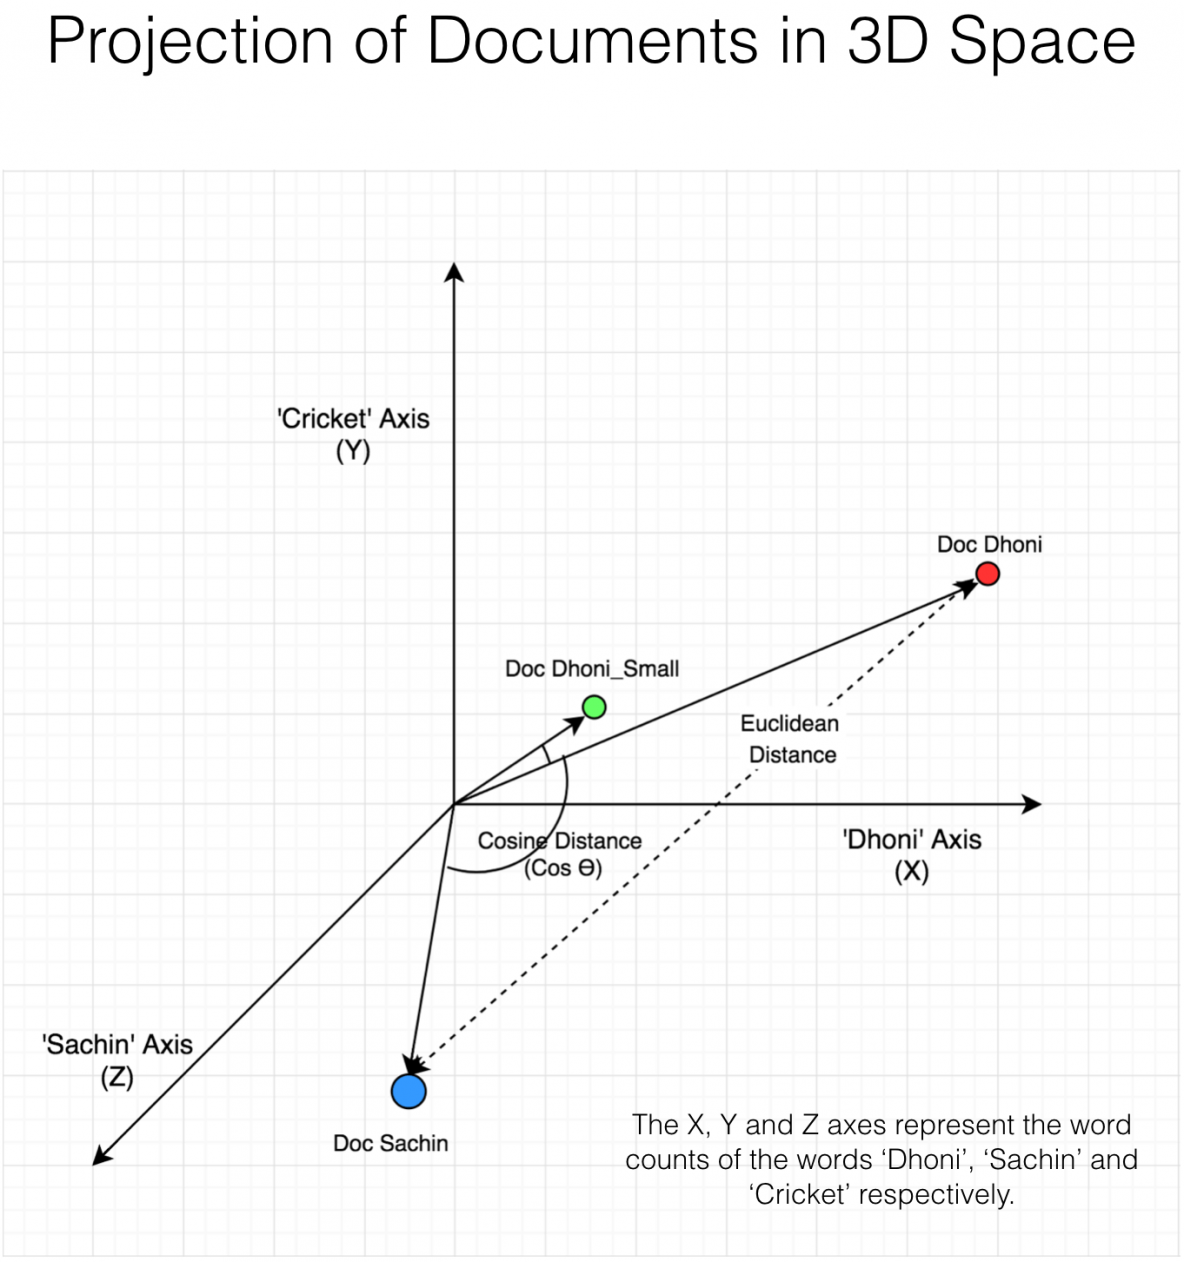
\includegraphics[scale=0.1]{images/placeholder_vectors}
    \caption{Cosine similarity use case}
    \label{fig:cosine_vectors}
\end{figure}

\noindent
As seen in figure \ref{fig:cosine_vectors} the red and blue vectors are closest by magnitude however by ignoring magnitude and just looking at angle the red vector is considered to be related to green. When a word appears in different contexts, its vector gets moved in different directions during updates. The final vector then represents some sort of weighted average over the various contexts. 

\section{Word Depth} 
The definition of word depth used here is in reference to semantic lexicons, these semantic lexicons are made up of entities. Each lexical entity is connected by semantic relations. In WordNet, entities with multiple meanings (synonymous) are grouped into what it calls synsets. WordNet is a lexical database project from Princeton University which includes four categories noun, verbs, adverbs and adjectives. When comparing noun and verb depth it is required to look at how WordNet data is organised into hierarchies. These hierarchies are created through the use of hypernyms. \textit{Y is a hypernym of X if every X is a (kind of) Y.} Noun hierarchies are far deeper than verb hierarchies.

This depth difference can disrupt matching when preforming similarity queries in WordNet. With nouns having having a deeper tree of hypernyms than verbs, it is more likely when comparing similarity between nouns a higher value will be found. This problem of word depth extends to other methods also, when preforming cosine similarity queries in Word2vec a more diverse range of scores is found when using nouns as opposed to verbs. Another factor that affect these scores in Word2vec is the lack of part of speech tagging (POS) in Word2vec.

\section{Verb Group sets}
Grouping words based around a specific category is often a difficult task, with verbs defined as action words one such grouping is commonly used by information professionals. Bloom's Taxonomy is centered around learning objectives and is structured as a hierarchy containing six categories. Within each of these categories verbs are used to define the learning objective.

\begin{figure}[H]
\centering
  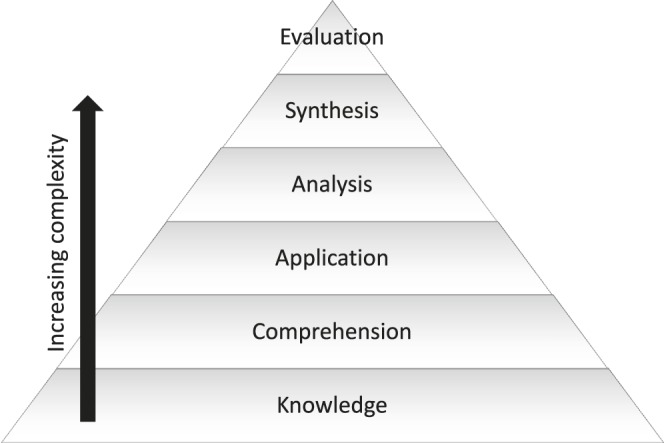
\includegraphics[width=\textwidth]{images/bloom.jpg}
  \caption{Bloom's Taxonomy}
  \label{fig:bloom}
\end{figure}

\noindent
By examining the verbs within each level it encourages instructors to think of learning objectives in behavioral terms to consider what the learner can do as a result of the instruction. \cite{Adams2015} Verbs within each category should have a high relational similarity as well as verbs between levels, with decreasing similarity the further the level away from the one being examined. As the complexity increases up the hierarchy actions or verbs within the evaluation category will require a much deeper understanding then those in the knowledge category.